\documentclass[12pt,a4paper,twoside]{book}


\usepackage[utf8]{inputenc}
\usepackage[a4paper,inner=3.5cm,outer=2.5cm]{geometry}

\usepackage[titletoc,title,toc,page]{appendix}
\usepackage{verbatim}
\usepackage{placeins}
\usepackage{hyperref}
\usepackage[italian]{babel}
\usepackage{tikz}
\usepackage{parskip}
\usepackage{acronym}
\usepackage{graphicx}
\usepackage{blindtext}
\usepackage{chngcntr}
\usepackage{url}
\counterwithin{table}{chapter}

\usepackage{newlfont}
\usepackage{fancyhdr}
\usepackage{listings}
\lstset{
    basicstyle=\color{white}\small\ttfamily,
    breaklines=true,
    frame=single,
    captionpos=b,
    backgroundcolor=\color{black},
    commentstyle=\color{gray},
    showstringspaces=false
}
\usepackage{indentfirst}
\usepackage[utf8]{inputenc}
\usepackage{float}
\usepackage{hyperref}
\usepackage[capitalize,noabbrev]{cleveref}
\usepackage{soul}
\usepackage[font=footnotesize,labelfont=bf]{caption}
\usepackage{setspace}
\usepackage{multirow}
\usepackage{hyphenat}
\hyphenation{mate-mati-ca recu-perare}

\usepackage{lscape} 

\usepackage{natbib}
\bibliographystyle{plainurl}
\setcitestyle{super,open={[},close={]}}

\newcommand{\rom}[1]{\uppercase\expandafter{\romannumeral #1\relax}}

\usepackage{pdfpages}

\acrodef{BGP}[BGP]{Border Gateway Protocol}
\acrodef{AS}[AS]{Autonomous System}
\acrodef{ASN}[ASN]{Autonomous System Number}
\acrodef{RPKI}[RPKI]{Resource Public Key Infrastructure}
\acrodef{EGP}[EGP]{Exterior Gateway Protocol}
\acrodef{SDN}[SDN]{Software Defined Networking}
\acrodef{ISP}[ISP]{Internet Service Provider}
\acrodef{BGPSec}[BGPSec]{Border Gateway Protocol Security}
\acrodef{RIS}[RIS]{Ripe Information Service}
\acrodef{RIR}[RIR]{Regional Internet Registry}
\acrodef{OSPF}[OSPF]{Open Shortest Path First}
\acrodef{IOS}[IOS]{Internetworking Operating System}
\acrodef{VLAN}[VLAN]{Virtual Local Area Network}
\acrodef{CAIDA}[CAIDA]{Cooperative Association for Internet Data Analysis}
\acrodef{IR}[IR]{Internal Router}
\acrodef{BR}[BR]{Border Router}
\acrodef{LXC}[LXC]{LinuX Container}
\acrodef{VM}[VM]{Virtual Machine}
\acrodef{VMM}[VMM]{Virtual Machine Monitor}
\acrodef{FRR}[FRR]{Free Range Routing}
\acrodef{RIP}[RIP]{Routing Information Protocol}
\acrodef{IGP}[IGP]{Interior Gateway Protocol}
\acrodef{EGP}[EGP]{Exterior Gateway Protocol}
\acrodef{SPoF}[SPoF]{Single Point of Failure}
\acrodef{IANA}[IANA]{Internet Assigned Numbers Authority}
\acrodef{NRO}[NRO]{Number Resource Organization}
\acrodef{IETF}[IETF]{Internet Engineering Task Force}

\begin{document}
% Per spostare i vari elementi più su o più giù gioca con i valori di vspace che ci sono tra uno e l'altro
\pagestyle{empty}
\newgeometry{
    left=20mm,
    right=20mm,
    top=20mm,
    bottom=20mm
}

\begin{titlepage}

\begin{center}

% marchio di ateneo

\includegraphics[width=6.5cm,height=4.7cm]{img/marchio-di-ateneo.png}

\vspace{10mm}

% \large is 12pt
{\large{\bf{Dipartimento di Informatica - Scienza e Ingegneria}}} 

\vspace{5mm}

% \Large is 14.4pt
{\Large{\bf{Corso di Laurea in Ingegneria e Scienze Informatiche}}}

\vspace{15mm}

{\Huge{\bf Analisi e Mitigazione delle Vulnerabilità nel Protocollo BGP: }\\
\vspace{3mm}
{\Huge{\bf  Un Approccio al Rafforzamento della Sicurezza nelle Reti di Telecomunicazioni}}\\
\vspace{3mm}}

\end{center}

\vspace{10mm}

\begin{minipage}[t]{0.40\textwidth}
{\Large{\bf Relatore: \\ Chiar.mo Prof.\\ Andrea Piroddi}}

\vspace{3mm}

\end{minipage}
\hfill
\begin{minipage}[t]{0.40\textwidth}\raggedleft
{\Large{\bf Presentata da: \\ Roberto Pisu}}
\end{minipage}

\vspace{30mm}

\rule[0.5cm]{15.8cm}{0.6mm}

\begin{center}
{\large{\bf Sessione Ottobre 2025 \\}}
{\large{\bf Anno Accademico 2024/2025\\}}
\end{center}

\end{titlepage}

\restoregeometry
\newpage
\begin{center}
    (DA FARE ALLA FINE)\\
    5 parole chiave per caratterizzare il contenuto della dissertazione:\\ (se non ti piacciono così sparse puoi anche semplicamente scriverle su una riga sola)
\end{center}

% https://tex.stackexchange.com/questions/26538/words-scattered-randomly-in-on-coverpage
\begin{tikzpicture}[overlay,remember picture,shift=(current page.center)]
\pgfmathsetseed{3}


\foreach [count=\count] \word in {Parola 1, parola 2, parola 3, parola 4, parola 5} {
\node [
    xshift={(mod(\count,3)-1)*(\paperwidth/4)},
    yshift={(mod(\count,7)-3)*(\paperwidth/6)},
    xshift=rand*4cm,
    yshift=rand*2cm,
    % rotate=rand*35,
    % opacity=rnd*0.5+0.125,
    font=\large] {\word};
}
\end{tikzpicture}
\newpage

\topmargin=6.5cm
\begin{flushright}
\emph{
\LARGE{Alla mia famiglia}\\\vspace{2mm}
\LARGE{ai miei amici e a chi mi è stato accanto.}\\\vspace{3mm} 
\LARGE{Che questo traguardo sia solo l'inizio.} 
}
\end{flushright}
\newpage~\newpage
\pagenumbering{gobble}
\chapter*{Abstract}
Abstract qui (ti consiglio di farlo alla fine)

\topmargin=-1cm
\tableofcontents
\thispagestyle{empty}
\listoftables
\thispagestyle{empty}
\listoffigures
\thispagestyle{empty}
\newpage~\newpage


\pagenumbering{arabic}
\setcounter{chapter}{-1}
\raggedbottom
\chapter{INTRODUZIONE} \label{chap:intro}
\pagestyle{plain}
\setcounter{page}{1}
\onehalfspacing

Al giorno d'oggi, Internet rappresenta una delle infrastrutture più critiche e pervasive della nostra società, in quanto viene utilizzata costantemente in molteplici ambiti della vita quotidiana: dalla comunicazione personale e professionale che ci tiene connessi a livello globale, all'accesso immediato a una quantità crescente di informazioni e contenuti multimediali, fino alla gestione di transazioni economiche, servizi bancari, amministrazione pubblica e logistica internazionale.

Semplificando, Internet può essere definita come la “rete delle reti”: una struttura complessa e gerarchica che consente il collegamento tra milioni di reti locali eterogenee, distribuite in tutto il mondo. A livello architetturale, Internet è composta da un numero elevato, ma finito, di \ac{AS}, ciascuno dei quali corrisponde a una rete di proprietà e gestione unificata — come ad esempio un \ac{ISP}, un’azienda, un’università o un ente governativo — caratterizzata da una propria politica di routing indipendente. \\
(Si stima l'esistenza di più di 90.000 \ac{AS} )

Per “politica di routing” si intende l’insieme di regole, preferenze e vincoli che determinano in che modo il traffico di rete viene instradato all’interno dell’\ac{AS} e verso gli altri sistemi autonomi. Il protocollo di routing incaricato di gestire la propagazione delle informazioni tra \ac{AS} è il \ac{BGP}, attualmente considerato lo standard de facto per l’interconnessione a livello globale. Il suo compito è annunciare e apprendere rotte \footnote{Una rotta è il percorso scelto dal protocollo di routing per raggiungere una rete specifica.}
, determinando così i percorsi lungo i quali i pacchetti viaggiano da un’estremità all’altra del mondo.

Nonostante la sua centralità e longevità, il protocollo \ac{BGP} presenta una serie di limiti strutturali, legati al fatto che fu progettato in un’epoca in cui la sicurezza informatica non era ancora una priorità. \ac{BGP} si basa infatti su un modello di fiducia implicita tra gli operatori di rete e non prevede, nella sua implementazione standard, meccanismi di autenticazione, integrità o verifica delle informazioni propagate. Questa mancanza di sicurezza nativa rende il protocollo vulnerabile a diversi tipi di attacco, tra cui il \textit{prefix hijacking}, il \textit{route leaking} e il \textit{session hijacking}, che possono compromettere seriamente l'affidabilità e la sicurezza della rete Internet.

Alla luce di queste considerazioni, risulta fondamentale analizzare in dettaglio il funzionamento di \ac{BGP} e le sue vulnerabilità, al fine di individuare le possibili contromisure per prevenire o limitare gli effetti di un eventuale attacco. In un mondo sempre più dipendente dall'utilizzo di Internet, garantire la resilienza e la sicurezza del protocollo di routing interdominio è una priorità non solo tecnica, ma anche strategica e geopolitica.

La tesi si compone di sette capitoli suddivisi come segue:

\begin{itemize}
    \item \textbf{Primo Capitolo - Autonomous System} Nel primo capitolo viene approfondito il ruolo dell'\ac{AS}, le sue caratteristiche, a cosa serve, come vengono classificati e altre informazioni utili a comprendere il funzionamento del protocollo \ac{BGP}.
    \item \textbf{Secondo Capitolo - Protocollo di routing BGP 4.0} In questo capitolo viene analizzato in dettaglio il funzionamento del protocollo \ac{BGP} (Border Gateway Protocol), attualmente lo standard principale per il routing tra sistemi autonomi su Internet. Dopo una panoramica introduttiva sui concetti fondamentali di routing, viene descritto il contesto storico e tecnico che ha portato all’introduzione di BGP, in particolare come evoluzione del precedente \ac{EGP}. Viene poi approfondita la natura del protocollo, la sua collocazione nei livelli del modello di rete e le dipendenze da altri protocolli sottostanti.
    Una sezione centrale del capitolo è dedicata al funzionamento interno di BGP: vengono spiegati il meccanismo di routing basato su path vector, l'applicazione delle politiche di importazione ed esportazione delle rotte, gli attributi utilizzati per determinare il miglior percorso e le strategie per evitare la formazione di cicli.
    Il capitolo si conclude con una descrizione del formato dei messaggi BGP e delle sessioni di peering tra router (iBGP ed eBGP), per poi presentare un confronto tra le versioni storiche del protocollo e le novità introdotte nell’attuale versione 4.0.
    \item \textbf{Terzo Capitolo - Metodologie di attacco e prevenzione del protocollo BGP} Nel terzo capitolo vengono approfondite le principali vulnerabilità del protcollo \ac{BGP} nella sua ultima versione 4.0, ne vengono analizzate le cause, le modalità di esecuzione dell'attacco e le possibili conseguenze.
    Vengono trattati tre scenari d'attacco particolarmente rilevanti: il \textit{prefix hijacking}, in cui un \ac{AS} annuncia indebitamente prefissi IP altrui; il \textit{route leaking}, che comporta la diffusione impropria di rotte apprese da altri peer; e il \textit{session hijacking}, in cui un attore malevolo intercetta o falsifica la sessione \ac{BGP} tra due router.
    Per ciascun attacco vengono analizzati nel dettaglio il funzionamento tecnico, le ripercussioni sul traffico e le vulnerabilità specifiche che vengono sfruttate.
    Successivamente, il capitolo introduce due tecnologie progettate per aumentare la sicurezza di \ac{BGP}: \ac{BGPSec}, che fornisce autenticazione crittografica delle informazioni di routing tramite firme digitali basate su curve ellittiche (ECDSA), e \ac{RPKI}, un’infrastruttura a chiave pubblica che permette di validare l’autorità di un \ac{AS} ad annunciare un determinato prefisso IP. Vengono evidenziate le differenze tra le due soluzioni e i rispettivi ambiti di applicazione.

    Nella parte finale, viene trattato il tema del monitoraggio delle anomalie \ac{BGP} attraverso piattaforme pubbliche come \textit{BGPStream} (di \ac{CAIDA}), \textit{RIPE RIS} e \textit{Route Views}, strumenti fondamentali per l’analisi forense, la diagnosi di incidenti e l’early warning \footnote{L'early warning è la capacità di rilevare tempestivamente anomalie o potenziali attacchi alla rete.} nel routing globale.
    
    \item \textbf{Quarto Capitolo - Implicazioni degli attacchi BGP nel mondo} Questo capitolo analizza due noti casi reali di attacchi al protocollo \ac{BGP}, con l’obiettivo di mostrare le conseguenze concrete che vulnerabilità teoriche possono avere su scala globale. Il primo caso è quello del \ac{BGP} hijacking da parte di Pakistan Telecom nel 2008, che causò l’inaccessibilità mondiale di YouTube per diverse ore. Il secondo riguarda China Telecom, coinvolta in episodi di deviazione di traffico internazionale tra il 2010 e il 2018.
        
    
    \item \textbf{Quinto Capitolo - Tecnologie utilizzate}
    Nel quinto capitolo entriamo nel vivo della simulazione, vengono infatti presentate le principali tecnologie adottate per costruire l’ambiente virtuale necessario alla simulazione degli attacchi e delle contromisure al protocollo \ac{BGP}. L’infrastruttura è basata su \ac{VM} Ubuntu Server create con VMware Workstation Pro, che sfrutta virtualizzazione hardware di tipo 2 (hosted) con supporto alla full virtualization assistita da hardware.

    All’interno di ogni VM vengono eseguiti container LXC, impiegati per simulare i router interni (\ac{IR}) in modo efficiente. Per la gestione del routing interno è stato utilizzato \ac{FRR}, mentre per i router di confine (\ac{BR}) è stato adottato GoBGP, particolarmente adatto alla configurazione delle sessioni \ac{BGP} e alla sperimentazione di meccanismi come \ac{RPKI} e \ac{BGPSec}.

    La rete complessiva è strutturata secondo una topologia a maglia parziale tra sette \ac{AS}, ciascuno dotato di una struttura interna realistica composta da router, switch e VLAN. Tale configurazione permette di testare scenari di routing complessi in un ambiente controllato e riproducibile.
    \item \textbf{Sesto Capitolo - Sviluppo e implementazione}
    \item \textbf{Settimo Capitolo - Prospettive future: SDN e BGP}
\end{itemize}

\chapter{Autonomous System}
In questo capitolo, andiamo ad analizzare cos'è un \ac{AS}, il suo ruolo nel routing globale e la loro classificazione.

\section{Il ruolo dell'AS in Internet}
Un \ac{AS} è definito come un insieme di indirizzi IP e router sotto il controllo di una singola entità amministrativa, che adotta una politica id routing uniforme e coerente verso l'esterno.
Secondo l’\textit{RFC 1930} dell’IETF, un \ac{AS} è necessario ogniqualvolta un’organizzazione desideri definire delle regole di instradamento proprie e differenziate rispetto ad altri domini di routing, oppure quando intrattiene relazioni di peering con più fornitori di connettività a Internet.
Ogni \ac{AS} è identificato univocamente dal \ac{ASN}, assegnato da uno dei cinque \ac{RIR}. \cite{cloudflareAS} \cite{rfc1930}

\subsection{Cos'è il Regional Internet Registry}
I \ac{RIR} sono organizzazioni responsabili dell'assegnazione e della registrazione delle risorse numeriche di Internet all'interno di specifiche regioni geografiche del mondo.
Le risorse che i \ac{RIR} assegnano e registrano sono:
\begin{itemize}
    \item Indirizzi IP sia IPv4 che IPv6.
    \item \ac{ASN} usati per identificare gli \ac{AS}.
\end{itemize}
Le organizzazioni (come gli \ac{ISP}, grandi aziende, università, enti governativi, ecc.) che desiderano connettersi a Internet in modo indipendente (ovvero, operare il proprio \ac{AS}) e/o avere un blocco di indirizzi IP pubblico da gestire direttamente, devono richiedere queste risorse al \ac{RIR} competente per la loro area geografica.

Attualmente, esistono 5 \ac{RIR} a livello globale:
\begin{itemize}
    \item AfriNIC (Africa)
    \item ARIN (Nord America)
    \item LACNIC (America Latina e Caraibi)
    \item APNIC (Asia e Oceania)
    \item RIPE NCC (Europa, Medio Oriente e parti dell'Asia Centrale)
\end{itemize}
\begin{figure}[H]
    \centering
    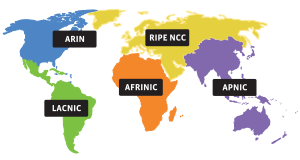
\includegraphics[width=.8\linewidth]{tesi/img/rir-map.png}
    \caption{Mappa dei RIR \cite{iana_RIR}}
    \label{fig:mappa_rir}
\end{figure}
Queste 5 \ac{RIR} collaborano attraverso l'\ac{NRO} e sono sotto la supervisione generale dell'ente \ac{IANA}, che è il coordinatore globale delle risorse numeriche e dei nomi di dominio di Internet. 

\subsection{Struttura ASN}
La nomenclatura degli \ac{ASN} segue due formati principali: il tradizionale a 16 bit e quello a 32 bit, introdotto successivamente per rispondere all’aumento della domanda (RFC 4893). Gli \ac{ASN} a 16 bit vanno da 1 a 65535, con alcune riserve speciali: per esempio, i numeri da 64512 a 65534 sono destinati all’uso privato, mentre l’\ac{ASN} 23456 viene usato come placeholder nella transizione tra 16 e 32 bit (RFC 6996). Il nuovo spazio a 32 bit estende la numerazione fino a 4.294.967.295 e consente anche l’utilizzo della notazione m:n (es. 1:10), che rappresenta una forma più leggibile del numero intero.

Gli \ac{ASN} vengono spesso preceduti dal prefisso AS (es: AS13335 per Cloudflare, AS15169 per Google) e sono registrati pubblicamente in database come il WHOIS. \footnote{WHOIS è un archivio pubblico che raccoglie informazioni sulla titolarità e sull'assegnazione di risorse di rete.} 
\cite{rfc6996}

\section{Classificazione AS}

Gli Autonomous System possono essere classificati secondo diversi criteri, in base al loro ruolo funzionale nella topologia globale di Internet, alla natura delle connessioni che intrattengono con altri \ac{AS}, oppure alle politiche di routing adottate.

Una classificazione comunemente diffusa è quella che distingue gli \ac{AS} in tre grandi categorie:
\begin{itemize}
    \item \textbf{Stub AS}: \ac{AS} che è connesso a uno o più provider, ma non fornisce connettività ad altri \ac{AS}. È il caso tipico di una rete aziendale o universitaria.
    \item \textbf{Multihomed AS}: \ac{AS} connesso a più provider, senza però fornire transito ad altri.
    \item \textbf{Transit AS}: \ac{AS} che offre connettività ad altri sistemi autonomi, permettendo loro di scambiare traffico. Gli \ac{ISP} operano tipicamente come transit \ac{AS}.
\end{itemize}

Un'altra classificazione si basa sul ruolo gerarchico ricoperto all’interno dell’ecosistema di Internet:
\begin{itemize}
    \item \textbf{Tier 1}: \ac{AS} che può raggiungere qualsiasi altra rete senza dover acquistare transito da altri AS.
    \item \textbf{Tier 2}: \ac{AS} che acquista transito, ma può anche offrire servizi a clienti e stabilire peering.
    \item \textbf{Tier 3}: \ac{AS} che acquista connettività esclusivamente da altri provider e non fornisce servizi di transito.
\end{itemize}

Infine, secondo le linee guida dell’\ac{IETF} (RFC 1930), un Autonomous System è definito anche in base all’autonomia decisionale rispetto alle politiche di routing. Questa indipendenza costituisce uno dei principali motivi per cui un’organizzazione può richiedere un \ac{ASN}.

\chapter{Protocollo di routing BGP 4.0}

\section{Cos'è il routing}

\section{Nascita del protocollo}

\subsection{Sostituzione EGP}

\section{Tipologia di protocollo (livello, a che altri protocolli di rete si appoggia)}

\section{Funzionamento BGP}

\subsection{Path vector}

\subsubsection{Come si applicano le politiche (import e export) policy}

\subsubsection{Attributi path vector}

\subsubsection{Come si evitano i cicli}

\subsection{Attributi BGP (a cosa serve ognuno)}

\subsection{Formato dei messaggi BGP}

\subsection{Sessioni BGP (eBGP, iBGP)}

\section{Differenze tra le varie versioni fino all'attuale 4.0}

\chapter{Metodologie di attacco e prevenzione del protocollo BGP}

\section{BGP prefix hijacking}

\subsection{funzionamento}

\subsection{conseguenze}

\subsection{che vulnerabilità sfrutta}

\section{BGP route leaking}

\subsection{funzionamento}

\subsection{conseguenze}

\subsection{che vulnerabilità sfrutta}

\section{BGP session hijacking}

\subsection{funzionamento}

\subsection{conseguenze}

\subsection{che vulnerabilità sfrutta}

\section{BGPSec}

\subsection{Come funziona BGPSec}

\subsection{Vulnerabilità risolte}

\subsection{Firma digitale con curve ellittiche (ECDSA)}
qui mi collego alla ricerca fatta con crittografia su ECDSA.

\section{BGP RPKI}

\subsection{Come funziona BGP RPKI}

\subsection{Vulnerabilità risolte}

\section{Monitoraggio e rilevamento anomalie}

\subsection{BGPStream (CAIDA)}

\subsection{CAIDA}

\subsection{RIPE RIS}

\subsection{Route Views}

\chapter{Implicazioni degli attacchi BGP nel mondo}

\section{BGP hijacking Pakistan Telecom 2008}

\section{BGP hijacking di China Telecom}

\chapter{Tecnologie utilizzate}
In questo capitolo, esamineremo le tecnologie scelte e il loro ruolo nella costruzione del progetto.

\section{Ambiente di virtualizzazione}
Data l'impossibilità di utilizzare, gratuitamente o a basso costo, dei router in grado di supportare \ac{BGPSec} e \ac{RPKI}, utilizzeremo delle \ac{VM} con sistema operativo Ubuntu server 24.04.2. Su queste \ac{VM}, monteremo poi dei software (FRRouting per i \ac{IR} e GoBGP per i \ac{BR}) per rendere le \ac{VM} dei router effettivi.

\subsection{VMware Workstation Pro}
Come software di virtulizzazione desktop per contenere le \ac{VM} utilizziamo VMware Workstation Pro nella sua versione 17.6.3. VMware Workstation Pro, nel 2024 è diventato gratuito nella sua versione per uso personale, e ciò ha contribuito ulteriormente nella sua diffusione, ad oggi esso è infatti uno dei software di virtualizzazione desktop più utilizzato. \cite{ionos2024}
Quando creiamo delle \ac{VM} con VMware Workstation Pro, usiamo la virtualizzazione hardware di tipo 2 (hosted) con full virtualization assistita da hardware.

\subsubsection{Terminologia della virtualizzazione}
\begin{itemize}
    \item \textbf{Sistema host}: è la macchina fisica su esegue il sistema operativo principale e che poi ospiterà le macchine virtuali.
    \item \textbf{Sistema guest}: è l'insieme delle risorse hardware e SO che viene eseguito "sopra" il sistema host.
    \item \textbf{Hypervisor o \ac{VMM}}: è il componente software che crea e manda in esecuzione le \ac{VM}. Ha il compito di astrarre e rendere disponibili le risorse hardware e svolge i compiti di monitoraggio e sicurezza.
\end{itemize}

\subsubsection{Virtualizzazione Desktop}
La virtualizzazione desktop, è un tipo di virtualizzazione che:
\begin{itemize}
    \item Consente di utilizzare una \ac{VM} che esegue sul PC dell'utente, in questo modo la macchina virtuale sfrutta le periferiche della macchina fisica (mouse, tastiera, schermo..) per consentire all'utente l'interazione con il sistema operativo guest.
    \item Viene realizzata mediante l'utlizzo di particolari software che permettono di eseguire altri sistemi operativi "sopra" il sistema operativo host.
    \item È utile per far funzionare un software non compatibile con il sistema operativo dell'host o un software che si vuole mantenere separato dal sistema operativo host.
\end{itemize}

\subsubsection{Virtualizzazione livello hardware}
Nella virtualizzazione livello hardware (macchine virtuali), all'utente del sistema di virtualizzazione viene presentata un'interfaccia su cui installare un sistema operativo, quindi una CPU virtuale (ma dello stesso tipo della CPU fisica) e risorse hardware virtuali.
Invece, nel caso di virtualizzazione livello di sistema operativo (container), all'utente viene presentata una partizione del sistema operativo correntre, su cui installare ed eseguire applicazioni che rimangono isolate nella partizione, pur accedendo ai servizi di uno stesso sistema operativo.
\begin{figure}[H]
    \centering
    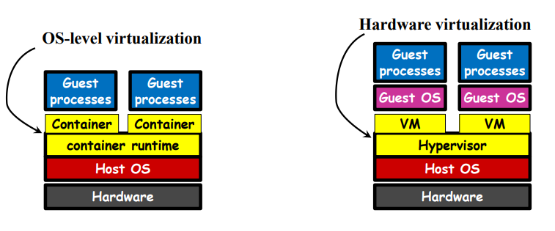
\includegraphics[width=.8\linewidth]{img/hardware-os_virtualization.png}
    \caption{OS virtualization VS Hardware virtualization}
    \label{fig:hardware-os_virtualization}
\end{figure}

\subsubsection{Virtualizzazione di tipo 2 (hosted)}
Si definisce virtualizzazione di tipo 2 o \textbf{hosted} un sistema di virtualizzazione nel quale l'hypervisor è un normale processo utente sul sistema operativo host. Mentre si definisce virtualizzazione di tipo 1 o \textbf{bare-metal} un sistema di virtualizzazione nel quale il sistema operativo host è assente e le sue funzioni vengono sostituite dall'hypervisor.
\begin{figure}[H]
    \centering
    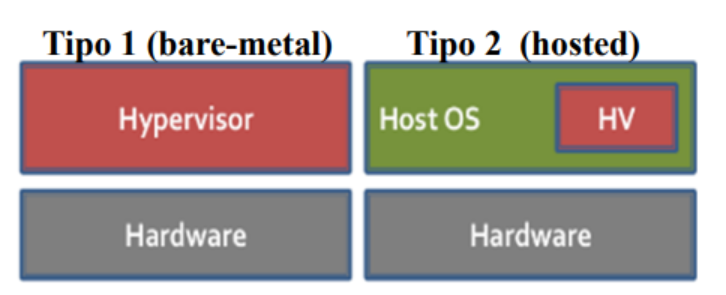
\includegraphics[width=.8\linewidth]{img/bare-metal_hosted.png}
    \caption{bare-metal vs hosted}
    \label{fig:bare-metal_hosted}
\end{figure}

\subsubsection{Virtualizzazione completa}
Nella virtualizzazione completa (o full virtualization), vengono fornite \ac{VM} che hanno la medesima interfaccia di una macchina fisica. Idealmente, il sistema operativo guest non può identificare che si trova su una macchina virtuale (in realtà di solito è sempre possibile dedurlo attraverso opportune teniche).
Invece, nella para virtualization la \ac{VM} presenta un'interfaccia diversa confrontata ad una macchina visica. Questo comporta dover modificare il sistema operativo guest per consentire l'esecuzione all'interno della macchina virtuale stess.

\begin{figure}[H]
    \centering
    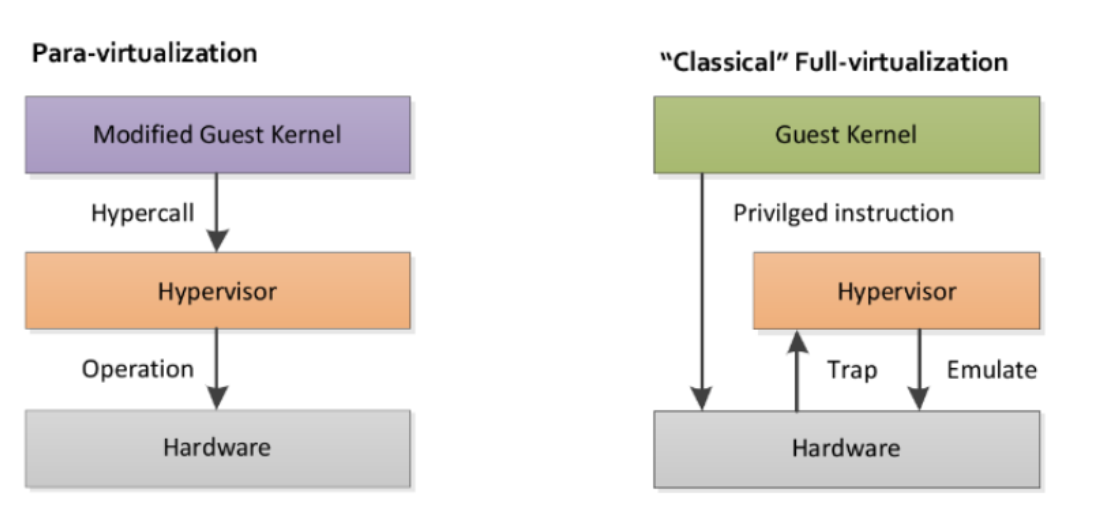
\includegraphics[width=.8\linewidth]{img/para-full_virtualization.png}
    \caption{para vs full virtualization}
    \label{fig:para-full_virtualization}
\end{figure}

\subsection{LXC}
Nel progetto, oltre all'utilizzo di macchine virtuali complete tramite VMware, si è resa necessaria una soluzione più leggera e scalabile per simulare un numero elevato di router appartenenti ai vari \ac{AS}.

\subsubsection{Cos'è LXC}
LXC (Linux Containers) è una tecnologia che permette di creare container Linux con un sistema operativo completo, isolati tra loro ma in grado di condividere lo stesso kernel Linux dell'host. A differenza delle \ac{VM}, i container LXC non virtualizzano l'intero hardware, ma sfruttano le funzionalità native del kernel come \texttt{cgroups} e \texttt{namespaces} per ottenere isolamento e gestione delle risorse.

Ogni container LXC può essere considerato una "mini-macchina Linux", capace di eseguire più processi, avviare demoni di sistema (come \texttt{systemd}) e simulare realisticamente il comportamento di un router software. Per questo motivo, è particolarmente adatto all’uso con \textbf{FRRouting}, in modo da trasformare ciascun container in un router.

\subsubsection{Motivazioni della scelta}
L’utilizzo esclusivo di \ac{VM} per ogni router avrebbe comportato la creazione e gestione di oltre 20 istanze complete di Ubuntu Server, con un notevole consumo di risorse hardware. LXC offre una soluzione molto più efficiente: consente di simulare decine di router su un'unica \ac{VM} host o macchina fisica, mantenendo un livello di realismo sufficiente per lo studio dei protocolli di routing.
In questo modo, andremo a creare 7 \ac{VM} ubuntu server, e su ognuna 4 \ac{LXC}.

\subsubsection{LXC vs Docker}
\begin{table}[H]
    \centering
    \label{tab:lxc-vs-docker}
    \renewcommand{\arraystretch}{1.3}
    \begin{tabular}{|p{4cm}|p{5cm}|p{5cm}|}
        \hline
        \textbf{Caratteristica} & \textbf{LXC} & \textbf{Docker} \\
        \hline
        Tipo di container & Container di sistema (full OS) & Container per singola applicazione \\
        \hline
        Sistema operativo & Completo, con supporto per \texttt{systemd}, più processi, demoni & Minimo, pensato per un processo alla volta; \texttt{systemd} non supportato nativamente \\
        \hline
        Architettura & Accesso diretto a kernel, cgroups, namespaces; somiglia a una VM leggera & Strato intermedio (Docker Engine); isolamento a livello applicativo \\
        \hline
        Facilità di configurazione & Più complesso, orientato a sysadmin & Semplice, pensato per sviluppatori e DevOps \\
        \hline
        Gestione dei processi & Più processi supportati nativamente & Singolo processo per container (multi-processo solo con workaround) \\
        \hline
        Rete & Networking avanzato con configurazioni personalizzabili (bridge, veth, ecc.) & Networking gestito dal motore Docker; meno flessibile \\
        \hline
        Supporto a demoni e init system & Completo (\texttt{systemd}, \texttt{init}, \texttt{cron}) & Limitato, solo con immagini o configurazioni speciali \\
        \hline
        Caso d’uso ideale & Simulare sistemi Linux completi (es. router, server reali) & Deploy di microservizi, app web, pipeline CI/CD \\
        \hline
        Ecosistema & Più ridotto, ma potente e vicino al kernel Linux & Ampissimo: Docker Hub, Docker Compose, Kubernetes \\
        \hline
    \end{tabular}
    \caption{Confronto tra LXC e Docker \cite{dockerLXC}} 
\end{table}

\subsubsection{Integrazione con VMware}
In questo progetto, LXC è stato utilizzato all’interno di una macchina virtuale host Ubuntu Server, eseguita su VMware. In questo modo si ottiene il vantaggio di una struttura modulare: le \ac{VM} rappresentano i confini tra gli \ac{AS}, mentre i container LXC al loro interno permettono di simulare in modo efficiente i router interni. I container sono interconnessi tramite bridge virtuali creati con \texttt{bridge-utils}, che permettono di emulare le reti locali tra gli \ac{IR} e gli \ac{BR} di ciascun \ac{AS}.

\paragraph{Vantaggi principali}
\begin{itemize}
    \item \textbf{Efficienza}: ogni container consuma pochi megabyte di RAM.
    \item \textbf{Realismo}: ambiente Linux completo, con supporto per FRRouting e configurazioni di rete avanzate.
    \item \textbf{Scalabilità}: facilità nel creare e clonare container per simulare topologie complesse.
    \item \textbf{Automazione}: possibilità di creare script per lanciare e configurare decine di router containerizzati.
\end{itemize}

\section{FRRouting}
\ac{FRR} è un software open-source che implementa numerosi protocolli di routing dinamico, tra cui \ac{BGP}, \ac{OSPF}, \ac{RIP} e altri. Nasce come fork di Quagga nel 2016, con l'obiettivo di offrire una suite più aggiornata, stabile e orientata alla produzione in ambienti carrier-grade, data center e reti ISP. \cite{frr-docs} 

FRRouting è scritto in C e si basa su una struttura modulare: ogni protocollo è gestito da un demone \footnote{dall'inglese \textit{deamon}, è un processo in background che opera in modo autonomo.} separato (es. \texttt{ospfd}, \texttt{bgpd}), coordinati dal demone \texttt{zebra}, responsabile dell'interazione con la tabella di routing del kernel Linux. La comunicazione tra i demoni avviene tramite un socket interno, e la configurazione può essere gestita tramite l'interfaccia a riga di comando \texttt{vtysh}.
Utilizzeremo l'ultima versione aggiornata a luglio 2025: la 10.3.1.

Nel progetto, FRRouting è utilizzato per trasformare i container LXC in veri e propri \ac{IR} interni all' \ac{AS}. In particolare, viene impiegato il protocollo OSPF per abilitare il routing interno all’\ac{AS} tra i router interni e il router di confine (\ac{BR}). Alcuni motivi per cui è stato scelto \ac{FRR} sono:
\begin{itemize}
    \item pieno supporto al protocollo OSPF;
    \item leggerezza e compatibilità con ambienti containerizzati (es. LXC);
    \item documentazione aggiornata e ampia community.
\end{itemize}
FRRouting è usato da numerosi operatori e progetti di rete, tra cui Cumulus Linux, VyOS, Google e altri attori del settore delle telecomunicazioni e dei data center \cite{openfrr2024}.

\section{GoBGP}
GoBGP è un'implementazione software del protocollo \ac{BGP} interamente sviluppata in Go. È stato progettato per essere un'applicazione \ac{BGP} moderna e flessibile, ideale per ambienti che richiedono scalabilità e automazione, come le infrastrutture \ac{SDN} e per testare funzionalità avanzate quali \ac{RPKI} e BGPsec. \cite{gobgp-docs}

GoBGP è un progetto open-source mantenuto dalla sua community, con il supporto attivo di contributori da NTT Communications e altri operatori. A differenza di molti altri router software, GoBGP adotta un'architettura "daemon-less": si tratta di un unico binario che include tutte le funzionalità. Questo lo rende gestibile in modo flessibile tramite API gRPC o file di configurazione in formato YAML o TOML \cite{gobgp-api}

Nel progetto, GoBGP viene utilizzato per configurare i router di confine (\ac{BR}) di ciascun \ac{AS} (in particolare utilizzeremo l'ultima versione aggiornata a luglio 2025: la 3.37.0). A differenza di FRRouting, GoBGP non implementa protocolli \ac{IGP} come OSPF o RIP, ma offre supporto avanzato per:
\begin{itemize}
    \item validazione \ac{RPKI} tramite RTR (RFC 6810/8210);
    \item supporto a BGPsec (in parte sperimentale);
    \item API per interazioni dinamiche e test automatizzati;
    \item capacità di annunciare/ritirare prefissi dinamicamente.
\end{itemize}

Questo rende GoBGP ideale per la simulazione di attacchi alla sicurezza di \ac{BGP} (es. prefix hijacking, route leaking) e per testare le contromisure basate su RPKI.

\section{Topologia rete}
Una topologia di rete descrive come i nodi e le connessioni sono organizzati, sia fisicamente che logicamente, all'interno di una rete.
Per il progetto è stata adottata una topologia fisica a maglia parziale, al fine di avvinarci maggiormente a ciò che avviene nella realtà. Mentre nella topologia a maglia completa tutti i nodi sono collegati tra loro, nella topologia a maglia parziale non tutti i nodi sono collegati.
Nella realtà, la topologia ha una struttura gerarchico-scalabile, in cui i grandi provider sono fortemente connessi tra loro, mentre i più piccoli hanno connessioni limitate verso l'alto.
Vediamo ora alcune caratteristiche di una topologia a maglia parziale:
\begin{itemize}
    \item ha una buona scalabilità \footnote{La scalabilità è la caratteristica di una rete di aggiungere o rimuovere nodi facilmente.}
    \item non tutti i nodi sono collegati tra loro, ma molti dispongono di connessioni multiple verso determinati nodi, ciò garantisce percorsi alternativi in caso di malfunzionamenti
    \item rispetto a una topologia a maglia completa, quella parziale più semplice da realizzare e meno costosa (banalmente perché richiede meno link fisici e meno hardware).
\end{itemize}

\subsection{Struttura rete generale (topologia a maglia parziale tra 7 AS)}
\begin{figure}[H]
    \centering
    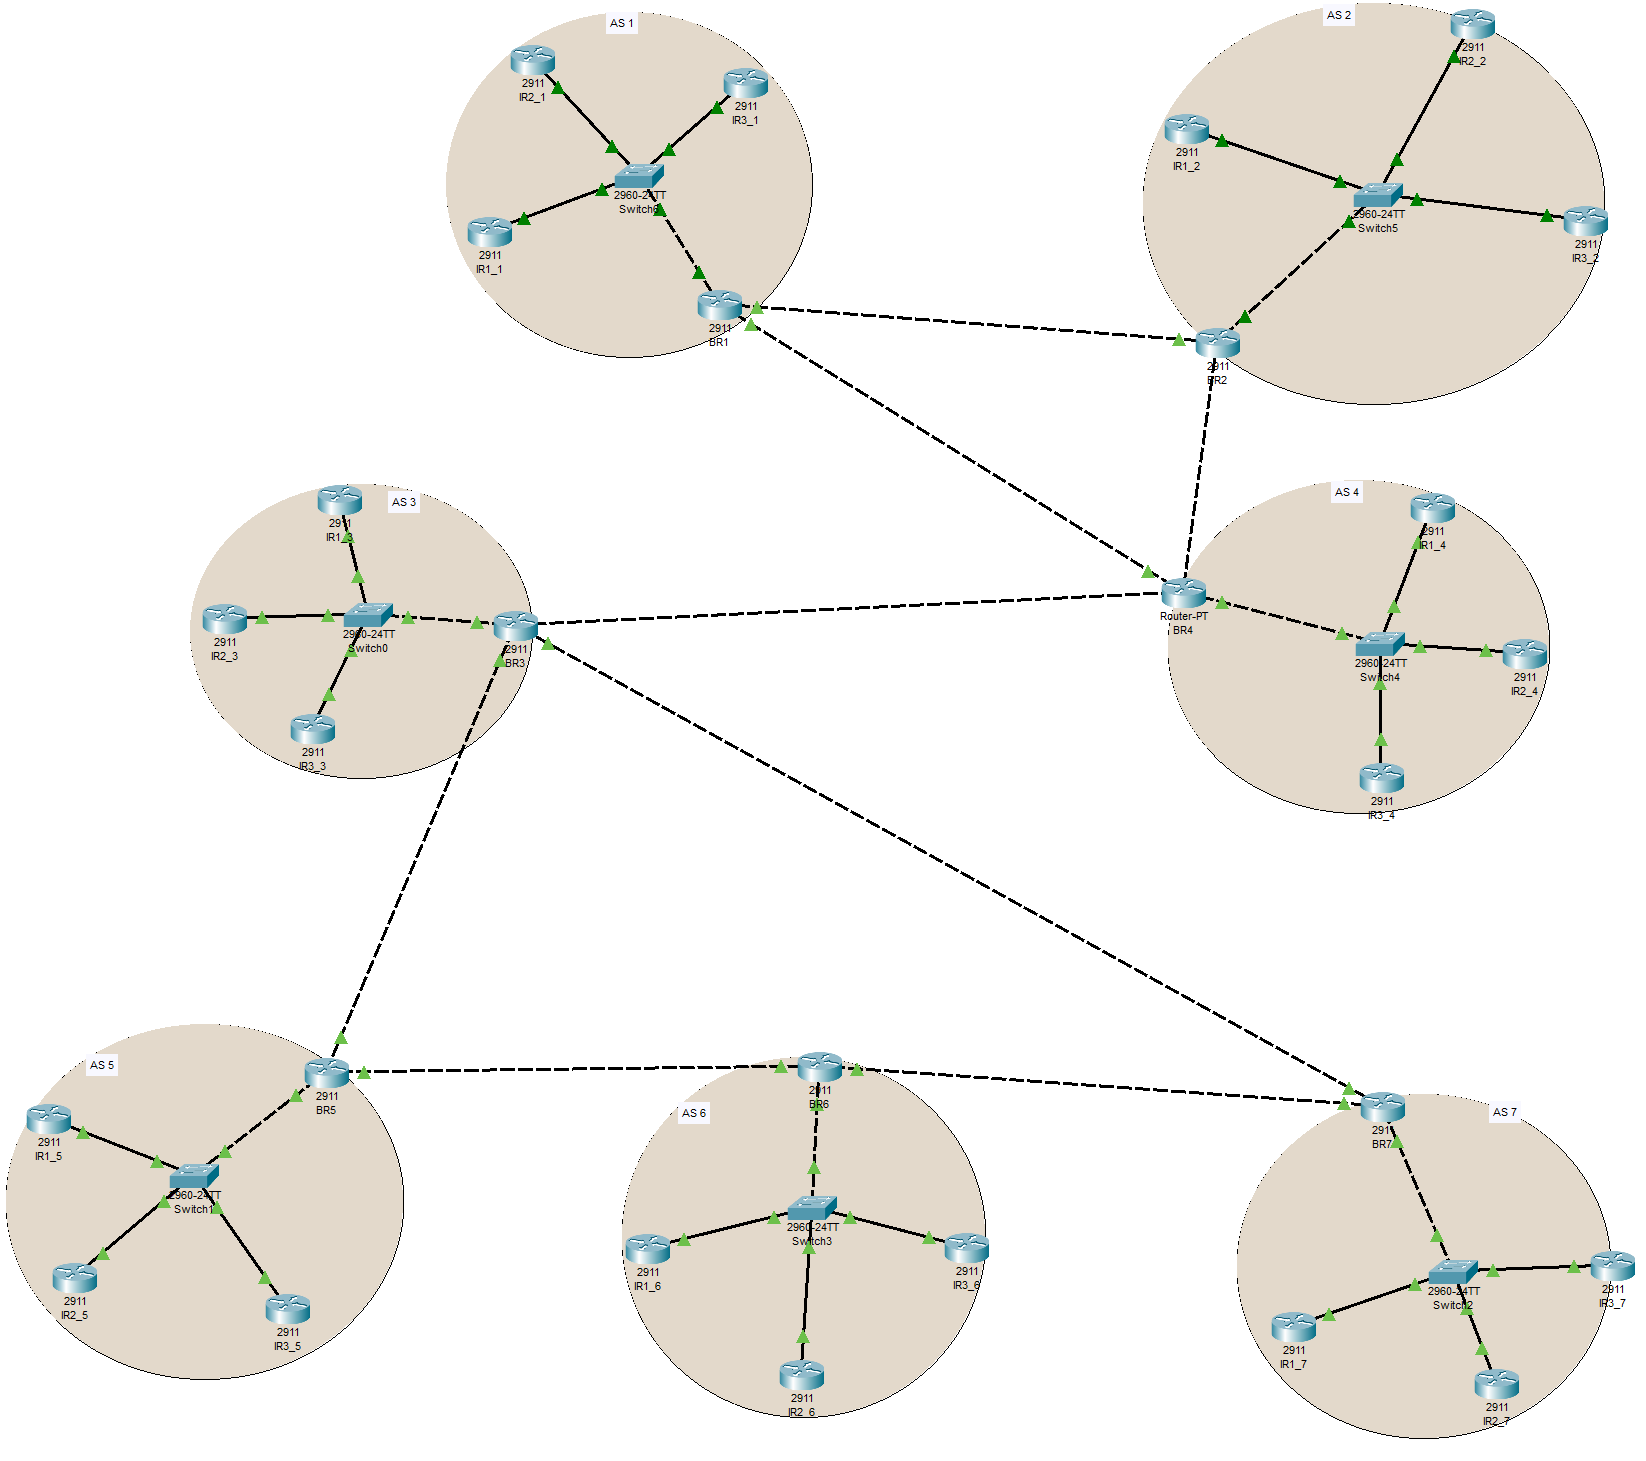
\includegraphics[width=.8\linewidth]{img/topologia_completa.png}
    \caption{Topologia della rete completa}
    \label{fig:topologia_completa}
\end{figure}

La rete è composta da sette \ac{AS}, ciascuno dotato di un proprio sistema interno di routing e di un \ac{BR} (router di confine). I \ac{BR} sono connessi tra loro secondo una topologia logica a maglia parziale, in cui ogni router di confine stabilisce connessioni \ac{BGP} soltanto con un sottoinsieme degli altri \ac{AS}.
I link \ac{BGP} tra \ac{BR} sono stati quindi progettati per formare una rete ridondata ma non simmetrica, garantendo percorsi alternativi senza replicare la connettività tra tutti i nodi.
Un approccio a simulazioni con questa topologia consente di osservare il comportamento del protocollo \ac{BGP} in scenari realistici, in cui le decisioni di instradamento devono tener conto di topologie non perfettamente connesse e della propagazione selettiva delle rotte.

\subsection{Stuttura singolo AS}
\begin{figure}[H]
    \centering
    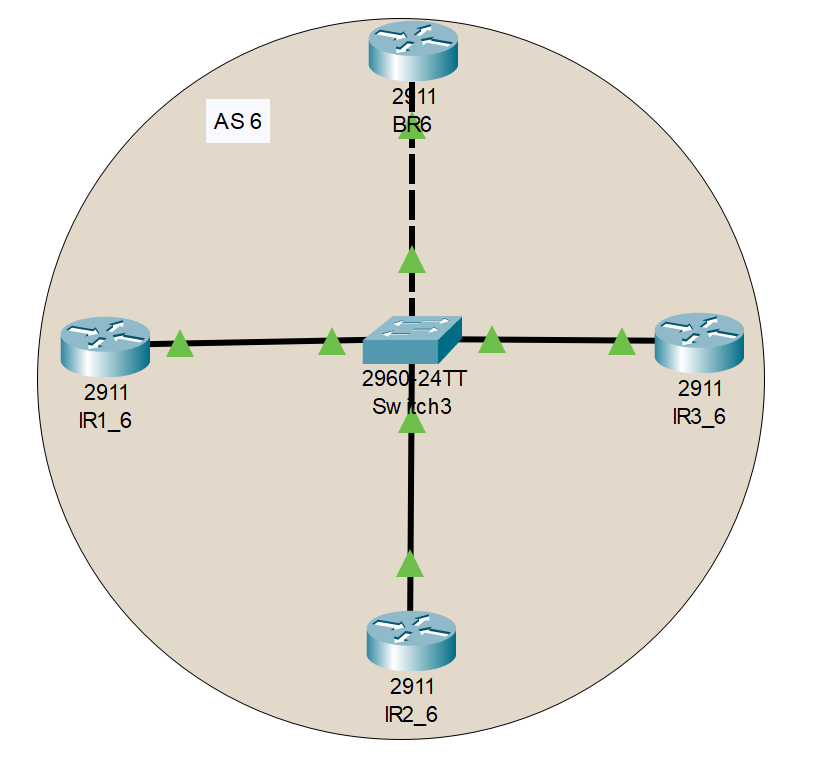
\includegraphics[width=.8\linewidth]{img/topologia_as.png}
    \caption{Topologia dell'AS}
    \label{fig:topologia_as}
\end{figure}
Ogni \ac{AS} è progettato con una struttura interna composta da moduli funzionali distinti (router interni, router di confine, switch e VLAN), pensata per simulare in modo realistico l’architettura di una rete aziendale. La composizione di ogni \ac{AS} è la seguente:

\begin{itemize}
    \item \textbf{1 \ac{BR}}: router di confine che comunica con gli altri \ac{BR} tramite il protocollo \ac{BGP}. È responsabile dell’interscambio delle rotte con l’esterno e dell’inoltro del traffico verso la rete interna dell’\ac{AS}.
    \item \textbf{3 \ac{IR}}: router interni all’\ac{AS}, collegati tra loro tramite un protocollo \ac{IGP}, in questo caso \ac{OSPF}. Gli \ac{IR} non comunicano direttamente con l’esterno, ma solo con il \ac{BR} e tra loro.
    \item \textbf{1 Switch Layer 2} configurato con \textbf{4 VLAN}:
    \begin{itemize}
        \item \textbf{3 VLAN dedicate}, ognuna per il collegamento tra un \ac{IR} e lo switch;
        \item \textbf{1 VLAN condivisa}, che collega i tre \ac{IR} e il \ac{BR}, consentendo il funzionamento del routing interno (\ac{OSPF}) tra tutti e quattro i router.
    \end{itemize}
\end{itemize}

\chapter{Sviluppo e implementazione}
In questo capitolo, vediamo tutti i passaggi pratici messi in pratica per realizzare l'ambiente di simulazione e i vari test alla sicurezza del protocollo \ac{BGP}.

\section{Creazione di un AS}
Ora vediamo i passi dettagliati per la creazione di un \ac{AS}, che ricordiamo essere composto da 3 \ac{IR} e 1 \ac{BR}. Inoltre abbiamo anche uno switch con 4 \ac{VLAN}: 3 \ac{VLAN} per ogni \ac{IR} e una \ac{VLAN} che permette ai 4 router di essere collegati tra loro e di gestire il routing tramite il protocollo \ac{OSPF}.

\subsection{Creazione VM con ubuntu server}
\begin{enumerate}
    \item Dal sito ufficiale di ubuntu: www.ubuntu.com, andiamo ad installare l'ultima versione della iso del sistema operativo ubuntu server.
    Nel mio caso l'ultima versione in data Giugno 2025 è: "ubuntu-24.04.2-live-server-amd64.iso".
    \item Avviamo VMware Workstation Pro e clicchiamo su “Create a New Virtual Machine”.
    \begin{figure}[H]
        \centering
        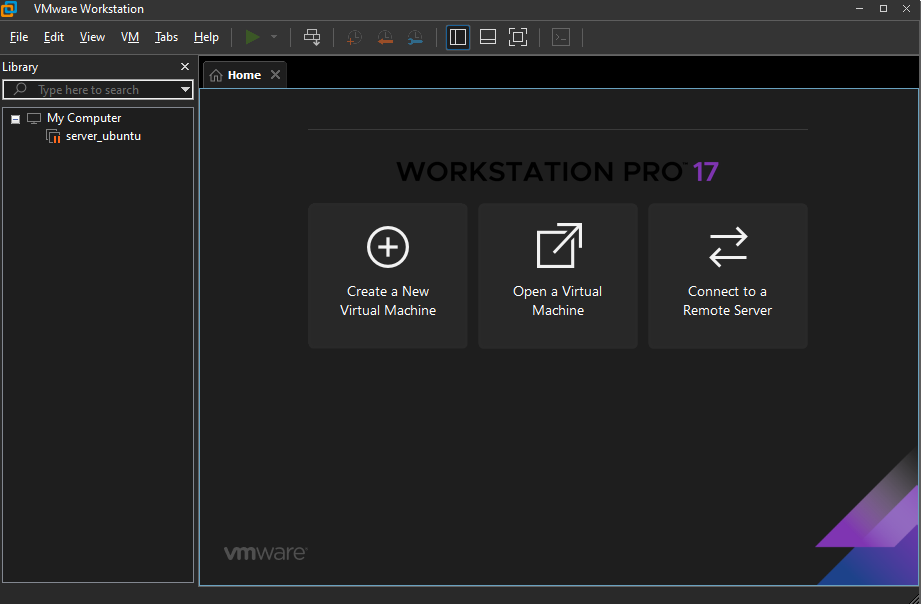
\includegraphics[width=.8\linewidth]{tesi/img/workstation_pro.png}
        \caption{Schermata di avvio di workstation pro 17}
        \label{fig:workstation_pro}
    \end{figure}
    \item Selezioniamo la iso precedentemente scaricata:
    \begin{figure}[H]
        \centering
        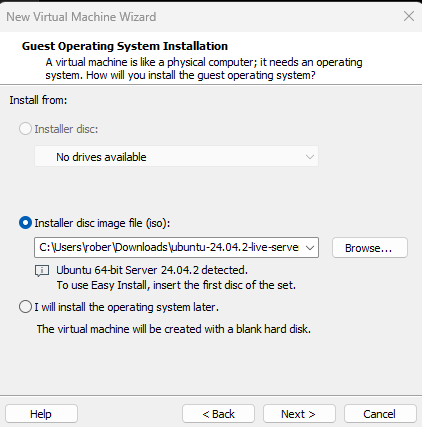
\includegraphics[width=.7\linewidth]{tesi/img/select_iso.png}
        \caption{Selezione file iso}
        \label{fig:select_iso}
    \end{figure}
    \item Gli diamo un nome e un percorso dove salvarla nel file system:
    \begin{figure}[H]
        \centering
        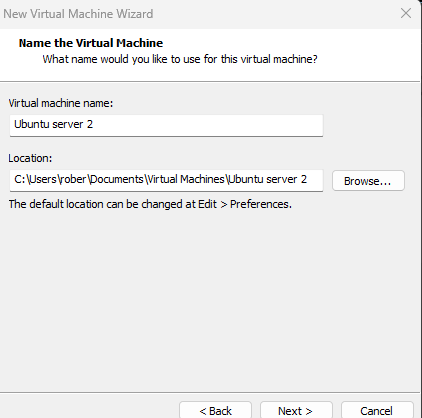
\includegraphics[width=.7\linewidth]{tesi/img/nome_percorso_VM.png}
        \caption{Nome e percorso VM}
        \label{fig:nome_percorso_VM}
    \end{figure}
    \item Specifichiamo 20 GB di archiviazione interna e l'opzione "Store virtual desk as a single file"
    \begin{figure}[H]
        \centering
        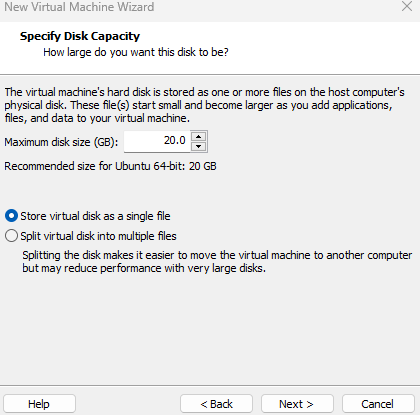
\includegraphics[width=.7\linewidth]{tesi/img/settings_VM.png}
        \caption{Impostazioni VM}
        \label{fig:settings_VM}
    \end{figure}
    \item A questo punto la configurazione è completa e si può avviare la macchina virtuale:
    \begin{figure}[H]
        \centering
        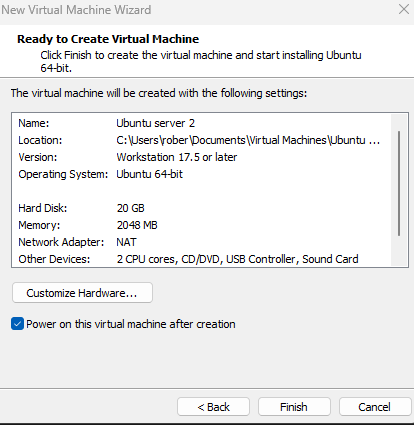
\includegraphics[width=.7\linewidth]{tesi/img/configurazione_VM_completa.png}
        \caption{VM completata}
        \label{fig:configurazione_VM_completa}
    \end{figure}
\end{enumerate}

\subsection{Configurazione ubuntu server}
Al primo avvio della macchina virtuale, il sistema operativo ubuntu server si configurerà in parte in automatico, mentre una parte della configurazione la dobbiamo completare noi manualmente:
\begin{enumerate}
    \item Selezioniamo la lingua di sistema e quella della tastiera:
    \begin{figure}[H]
        \centering
        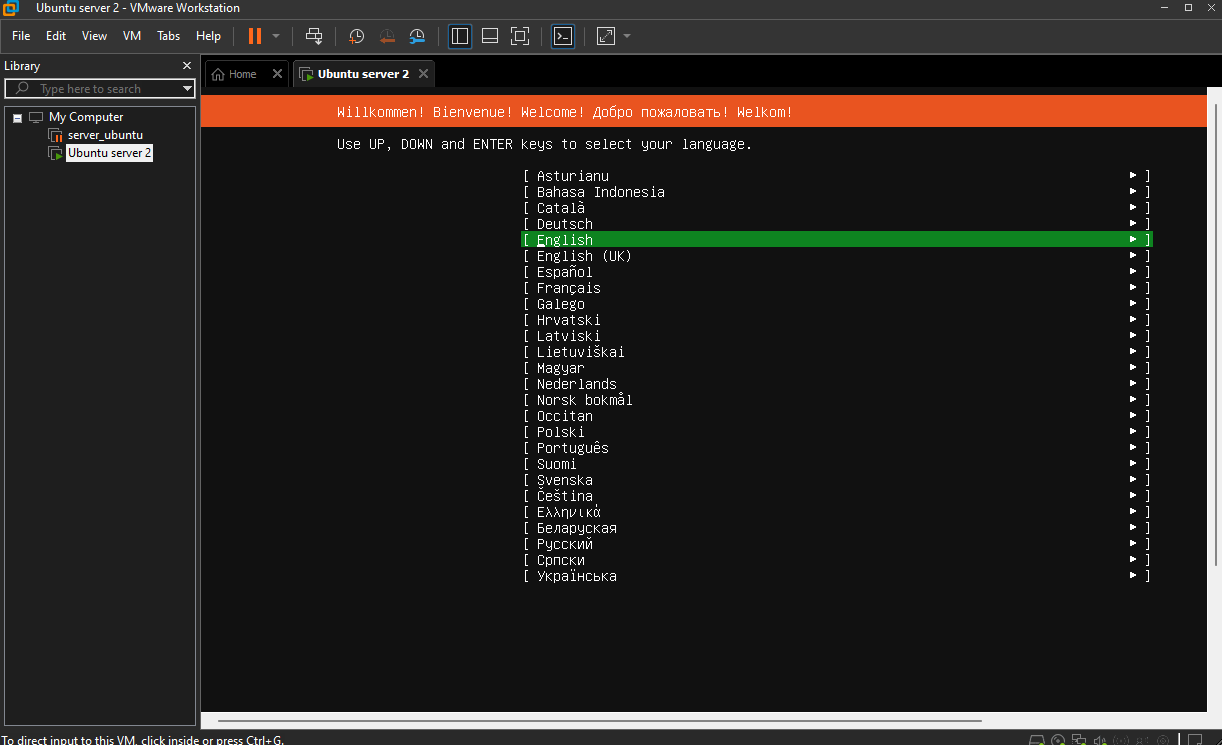
\includegraphics[width=.7\linewidth]{tesi/img/lingua_ubuntu.png}
        \caption{Selezione lingua}
        \label{fig:lingua_ubuntu}
    \end{figure}
    \item Scegliamo la modalità di installazione "minimized". La modalità minimized di una distribuzione Linux è una modalità più leggera rispetto a quella standard. \'E ideale al nostro contesto perché:
    \begin{itemize}
        \item riduce l'utilizzo di risorse della \ac{VM} (disco, RAM);
        \item è più semplice da configurare;
        \item evita software non necessario.
    \end{itemize}
      \begin{figure}[H]
        \centering
        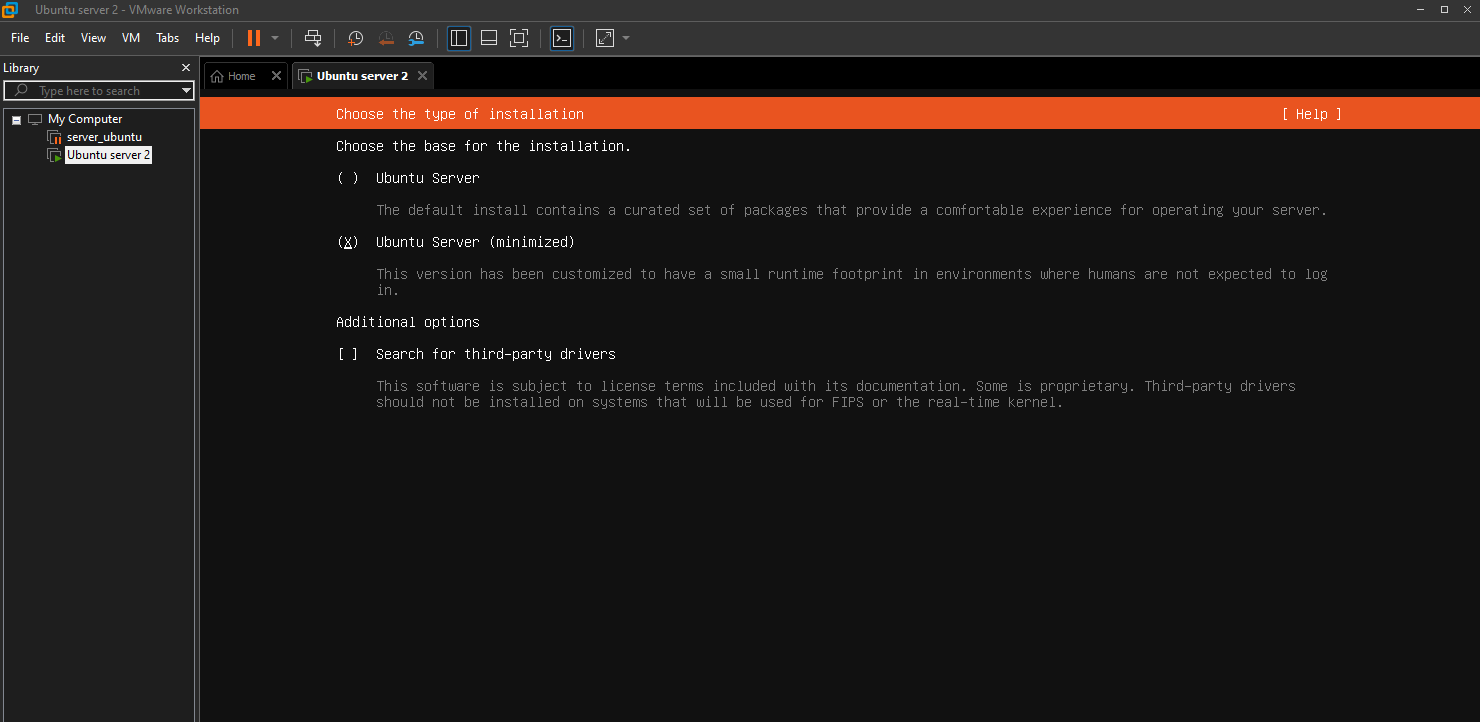
\includegraphics[width=.7\linewidth]{tesi/img/installazione_minimized.png}
        \caption{Ubuntu minimized}
        \label{fig:installazione_minimized}
    \end{figure}
    \item La configurazione della rete per ora la lasciamo così, la andremo a modificare in un secondo momento.
    \item La configurazione del proxy la lasciamo vuota.
    \item A questo punto ci viene chiesto quale mirror usare, lasciamo quello di default e andiamo avanti. Un mirror è un server che contiene una copia dell'archivio ufficiale di Ubuntu e serve principalmente a distribuire pacchetti del sistema operativo e dei software.
    \begin{figure}[H]
        \centering
        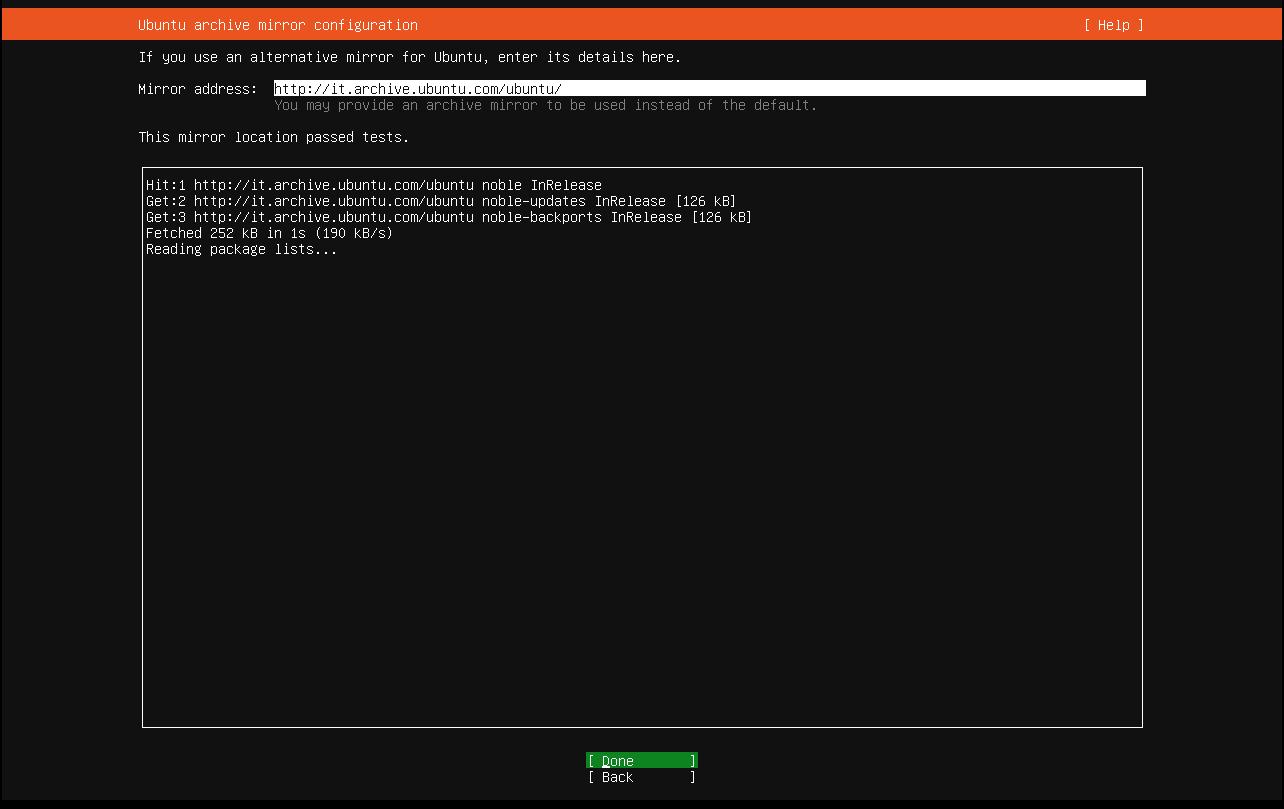
\includegraphics[width=.7\linewidth]{tesi/img/mirror_configuration.png}
        \caption{Configurazione mirror ubuntu}
        \label{fig:mirror_configuration}
    \end{figure}
    \item Per la configurazione storage lasciamo così com'è.
    \begin{figure}[H]
        \centering
        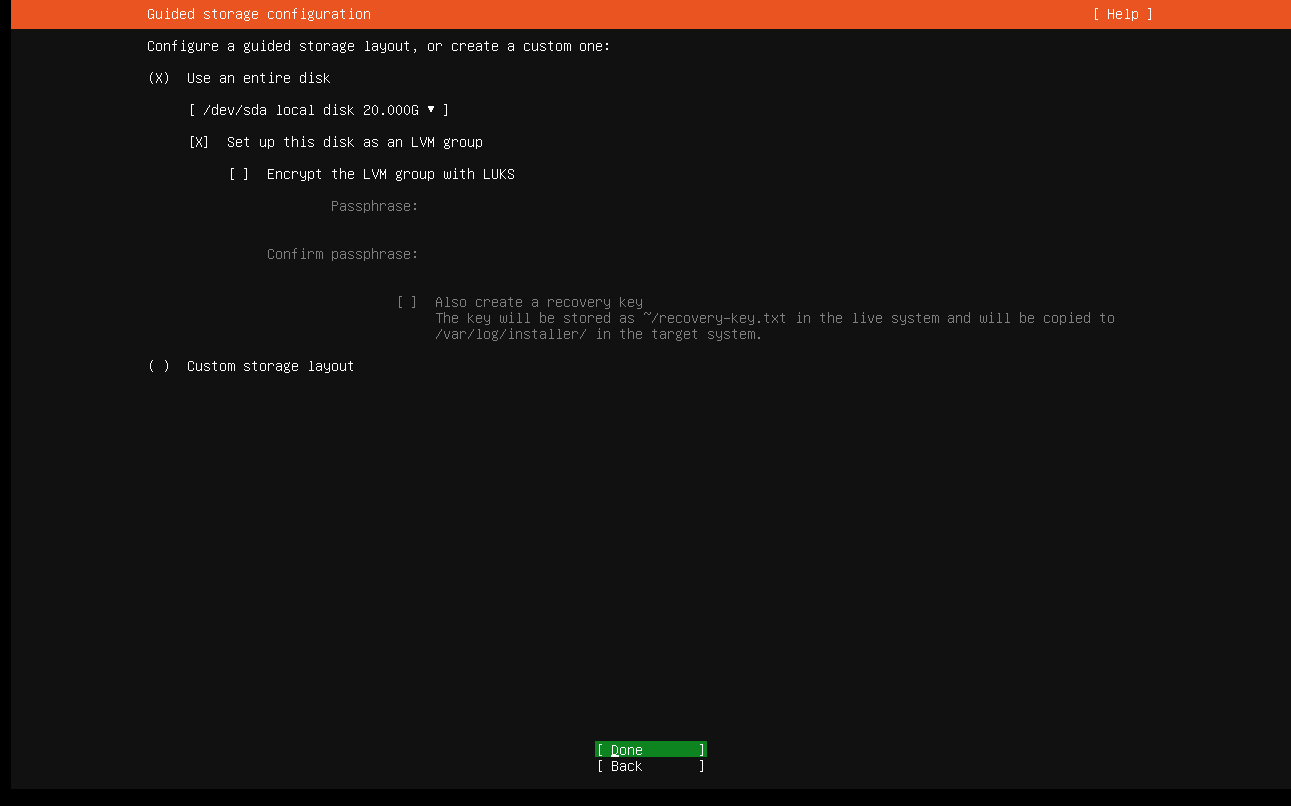
\includegraphics[width=.7\linewidth]{tesi/img/configurazione_storage.png}
        \caption{Configurazione storage}
        \label{fig:configurazione_storage}
    \end{figure}
    \item Ora ci viene chiesto di inserire username, nome del server, la password e il nome della macchina. Compiliamo i dati e andiamo avanti.
    \item Infine ci verrà chiesto di installare qualche software tra i più utilizzati e altre impostazioni che possiamo ignorare (lasciare tutto com'è di default e andare avanti). A questo punto, Ubuntu server minimized è installato sulla nostra \ac{VM} e pronto all'uso.
\end{enumerate}



\subsection{Installazioni preliminari sulla VM host}

\subsubsection{Installazione \ac{LXC} e dipendenze}
\begin{lstlisting}[language=bash]
$ sudo apt update
$ sudo apt install lxc bridge-utils net-tools -y
\end{lstlisting}
\subsubsection{Verifica se \ac{LXC} è configurato correttamente}
\begin{lstlisting}[language=bash]
$ lxc-checkconfig
\end{lstlisting}
Se lo è, darà in output tutte flag verdi con scritto "Enabled".
\subsubsection{Creazione container}
Ora creiamo i container che conterranno i router virtuali del nostro \ac{AS}. Avranno tutti sistema operativo Ubuntu 20.04 LTS a 64 bit.
\begin{lstlisting}[language=bash]
$ sudo lxc-create -t download -n ir1a -- -d ubuntu -r focal -a amd64
$ sudo lxc-copy -n ir1a -N ir1b
$ sudo lxc-copy -n ir1a -N ir1c
$ sudo lxc-copy -n ir1a -N br1
\end{lstlisting}
Verifichiamo che i container siano visibili:
\begin{lstlisting}[language=bash]
$ lxc-ls -f
\end{lstlisting}
Se lo sono, ci darà come output l'elenco dei nomi dei container con alcune caratteristiche.

\subsubsection{Creazione di bridge virtuali sulla VM host}
Per le 4 \ac{VLAN} interne, andiamo a creare 4 rispettivi bridge virtuali modificando il file "/etc/netplan/50-cloud-init.yaml" in questo modo:
\begin{figure}[H]
    \centering
    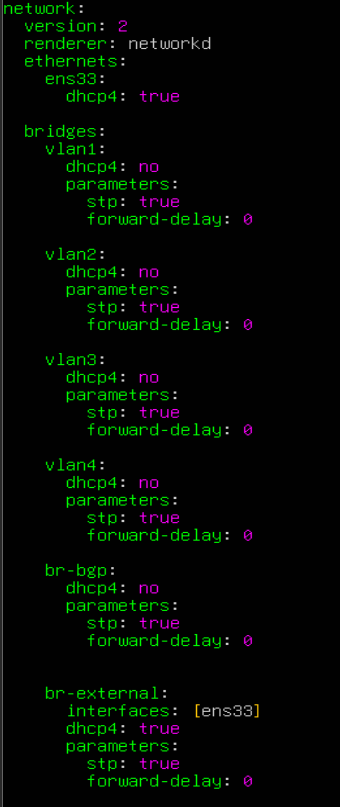
\includegraphics[scale=0.7]{tesi/img/creazione_bridge_virtuali.png}
    \caption{Configurazione bridge virtuali}
\label{fig:creazione_bridge_virtuali}
\end{figure}
e applichiamo la configurazione:
\begin{lstlisting}[language=bash]
$ sudo netplan apply
\end{lstlisting}

Una volta creati, li attiviamo:
\begin{lstlisting}[language=bash]
$ sudo ip link set vlan1 up
$ sudo ip link set vlan2 up
$ sudo ip link set vlan3 up
$ sudo ip link set vlan4 up
$ sudo ip link set br-bgp up
\end{lstlisting}

e assegnamo le interfacce dei container ai bridge.
Per ogni container andiamo a fare il comando:
\begin{lstlisting}[language=bash]
$ sudo nano /var/lib/lxc/<nome-container>/config
\end{lstlisting}
e li configuriamo come nell'immagine sottostante:
\begin{figure}[H]
    \centering
    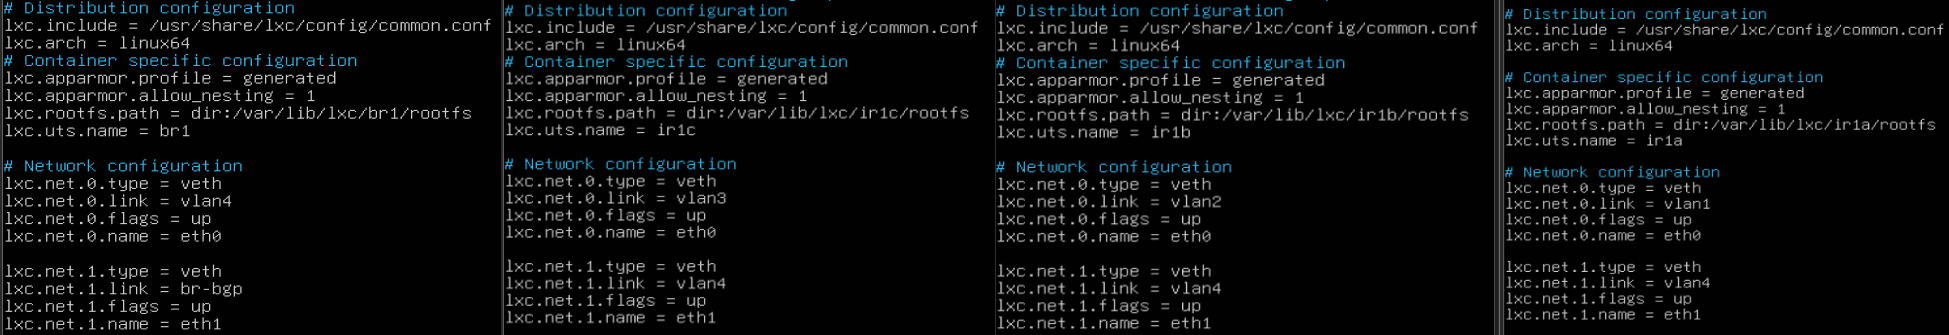
\includegraphics[width=1.0\linewidth]{tesi/img/configurazione_interfacce.png}
    \caption{Configurazione interfacce}
    \label{fig:configurazione_interfacce}
\end{figure}

\subsubsection{Avvio dei container}
Per ogni container andiamo ad eseguire:
\begin{lstlisting}[language=bash]
$ sudo lxc-start -n <nome-container>
\end{lstlisting}
E per controllare che tutti siano partiti correttamente:
\begin{lstlisting}[language=bash]
$ sudo lxc-ls -f
\end{lstlisting}

\subsubsection{Configurazione della rete nei router}
Per prima cosa entriamo nel container che rappresenta il nostro router (ad esempio: ir1a)
\begin{lstlisting}[language=bash]
$ sudo lxc-attach -n ir1a
\end{lstlisting}
Poi andiamo a modificare il file "10-lxc.yaml" di netplan \footnote{Netplan è un utility di configurazione di rete.}. Questo file conterrà la configurazione di rete per i bridge virtuali che verranno usati dai container \ac{LXC}.
\begin{lstlisting}[language=bash]
$ sudo nano /etc/netplan/10-lxc.yaml
\end{lstlisting}
E lo modifichiamo in questo modo:
\begin{lstlisting}[language=bash]
network:
  version: 2
  ethernets:
    eth0:
      addresses: [172.16.32.1/19]
    eth1:
      addresses: [172.16.128.2/19]
    eth2:
      dhcp4: yes
\end{lstlisting}
Poi per gli altri router abbiamo rispettivamente:
\begin{itemize}
    \item \textbf{ir1b}: 172.16.64.1, 172.16.128.3
    \item \textbf{ir1c}: 172.16.96.1, 172.16.128.4
    \item \textbf{br1}: 10.0.0.2 (esterna per \ac{BGP}), 172.16.128.5 (interna)
\end{itemize}

\subsubsection{Abilitiamo la connessione a internet a tutti i container}
Per scaricare i software necessari per rendere i nostri container dei router virtuali, è necessario che essi riescano ad accedere ad internet, per cui:
\begin{itemize}
    \item Nella \ac{VM} host, apriamo il file "/etc/netplan/50-cloud-init.yaml" e creiamo il bridge "br-external":
    \begin{figure}[H]
        \centering
        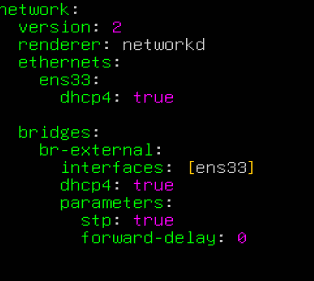
\includegraphics[width=.6\linewidth]{tesi/img/cloud-init-yaml.png}
        \caption{Configurazione rete VM host}
        \label{fig:cloud-init-yaml}
    \end{figure}
    Poi salviamo la configurazione:
    \begin{lstlisting}[language=bash]
sudo netplan apply
    \end{lstlisting}
    \item Abilitiamo il NAT sulla \ac{VM} host:
    \begin{lstlisting}[language=bash]
sudo nano /etc/sysctl.conf
    \end{lstlisting}
    e decommentiamo "net.ipv4.ip\_forward=1"
    \item Creiamo poi una regola NAT:
    \begin{lstlisting}[language=bash]
sudo iptables -t nat -A POSTROUTING -o br-external -j MASQUERADE
    \end{lstlisting}
    e facciamo in modo che si salvi anche al reboot:
    \begin{lstlisting}[language=bash]
sudo apt install iptables-persistent
sudo netfilter-persistent save
    \end{lstlisting}
    \item Aggiungiamo il bridge "br-external" nella configurazione di rete del container.
    Apriamo il file "\url{/var/lib/lxc/<nome-container>/config}" e aggiungiamo:
    \begin{lstlisting}[language=bash]
lxc.net.2.type = veth
lxc.net.2.link = br-external
lxc.net.2.flags = up
lxc.net.2.name = eth2
    \end{lstlisting}
    e poi riavviamo il container 
        \begin{lstlisting}[language=bash]
lxc-stop -n ir1a
lxc-start -n ir1a
    \end{lstlisting}
    \item Accediamo al container e diamo una configurazione dhcp all'interfaccia:
    \begin{lstlisting}[language=bash]
lxc-attach -n ir1a
dhclient eth2
    \end{lstlisting}
\end{itemize}
Ora il container ir1a è abilitato ad accedere a internet (possiamo testare con un semplice \textit{ping google.com}), ripetiamo questi passaggi per tutti gli altri container e possiamo andare avanti.


\subsection{Installazione FRR sui container}
Ora vediamo come installare \ac{FRR} sui container ai router:
\begin{itemize}
    \item Aggiorniamo l'indice dei pacchetti disponibili sui repository:
    \begin{lstlisting}[language=bash]
sudo apt update
    \end{lstlisting}
    \item Installiamo 3 tool che ci saranno utili: curl \footnote{Curl è un tool utile per scaricare file o interagire con API web da riga di comando.}, gnupg2\footnote{Gnupg2 fornisce un implementazione del software di crittografia OpenPGP, usato per verificare l'autenticità dei pacchetti.} e lsb-release\footnote{Tool che fornisce informazioni sulla distribuzione Linux in uso.}
    \begin{lstlisting}[language=bash]
sudo apt install -y curl gnupg2 lsb-release
    \end{lstlisting}
    \item Ora, siccome \ac{FRR} non è in un repository predefinito di linux, dobbiamo:
    \begin{itemize}
        \item scaricare una chiave pubblica GPG di \ac{FRR} con curl
        \item rendere questa chiave utilizzabile dal sistema Linux con "gpg --dearmor"
        \item installarla in un posto sicuro dove apt (il gestore dei pacchetti Ubuntu) la cercherà
    \end{itemize}
       \begin{lstlisting}[language=bash]
curl -s https://deb.frrouting.org/frr/keys.asc | sudo gpg --dearmor -o /usr/share/keyrings/frr.gpg
    \end{lstlisting}
    \item Ora aggiungiamo una nuova voce di repository per \ac{FRR} alla configurazione del gestore di pacchetti apt.
    \begin{lstlisting}[language=bash]
echo "deb [signed-by=/usr/share/keyrings/frr.gpg] https://deb.frrouting.org/frr/ $(lsb_release -cs) frr-stable" | sudo tee /etc/apt/sources.list.d/frr.list
    \end{lstlisting}
    \item Aggiorniamo nuovamente l'indice dei pacchetti disponibili sui repository:
    \begin{lstlisting}[language=bash]
sudo apt update
    \end{lstlisting}
     \item E finalmente installiamo \ac{FRR} e i suoi strumenti python:
    \begin{lstlisting}[language=bash]
sudo apt install frr frr-pythontools -y
    \end{lstlisting}
    \item Per testare se tutto l'installazione è avvenuta correttamente, il seguente comando deve mostrare la versione di \ac{FRR} installata:
    \begin{lstlisting}[language=bash]
vtysh -c "show version"
    \end{lstlisting}
\end{itemize}

\subsection{Installazione GoBGP sui container dei Border Router}
Invece, per installare GoBGP sui container dedicati ai \ac{BR}:
\begin{itemize}
    \item Aggiorniamo l'indice dei pacchetti disponibili sui repository:
    \begin{lstlisting}[language=bash]
sudo apt update
    \end{lstlisting}
    \item Installiamo i pacchetti wget\footnote{Tool da riga di comando per scaricare file da internet} e unzip\footnote{Tool da riga di comando per decomprimere file compressi in formato .zip.}:
    \begin{lstlisting}[language=bash]
sudo apt install wget unzip -y
    \end{lstlisting}
    \item Scarichiamo con wget l'ultima versione delll'archivio zip contenente l'eseguibile di GoBGP, prendendolo dal repository Github ufficiale del progetto.
    \begin{lstlisting}[language=bash]
wget https://github.com/osrg/gobgp/releases/download/v3.37.0/gobgp_3.37.0_linux_amd64.tar.gz
    \end{lstlisting}
    \item Decomprimiamo il file .tar.gz:
    \begin{lstlisting}[language=bash]
tar -xzf gobgp_3.37.0_linux_amd64.tar.gz
    \end{lstlisting}
    \item Spostiamo gli eseguibili "gobgp" e "gobgpd" estratti dall .tar.gz nella directory "/usr/local/bin/", in modo da poterli eseguire da qualsiasi posizione del terminale:
     \begin{lstlisting}[language=bash]
sudo mv gobgp gobgpd /usr/local/bin/
    \end{lstlisting}
    \item Infine controlliamo se abbiamo fatto tutto correttamente, controllando la versione di GoBGP:
     \begin{lstlisting}[language=bash]
gobgp --version
    \end{lstlisting}
\end{itemize}

\subsection{Configurazione OSPF nei router}
Per ogni router appartenente all'\ac{AS}, andiamo ora a configurare \ac{OSPF} in questo modo:
\begin{itemize}
    \item Avviamo il container:
    \begin{lstlisting}[language=bash]
lxc-start -n <nome-router>
    \end{lstlisting}
    \item Accediamo al container:
    \begin{lstlisting}[language=bash]
lxc-attach -n <nome-router>
    \end{lstlisting}
    \item Accediamo alla console del router:
    \begin{lstlisting}[language=bash]
vtysh
    \end{lstlisting}
    \item Entriamo nella modalità di configurazione avanzata:
    \begin{lstlisting}[language=bash]
conf t
    \end{lstlisting}
    \item Abilitiamo il processo \ac{OSPF}:
    \begin{lstlisting}[language=bash]
router ospf
    \end{lstlisting}
    \item Selezionamo l'interfaccia preposta per la vla4:
    \begin{lstlisting}[language=bash]
interface eth1
    \end{lstlisting}
    \item Colleghiamo l'interfaccia di rete alla backbone \ac{OSPF} (area 0):
    \begin{lstlisting}[language=bash]
ip ospf area 0
    \end{lstlisting}
    \item Usciamo dalla modalità di configurazione avanzata:
    \begin{lstlisting}[language=bash]
exit
    \end{lstlisting}
    \item E salviamo la configurazione:
    \begin{lstlisting}[language=bash]
write
    \end{lstlisting}
    \item Per vedere se i vicini ospf sono corretti:
    \begin{lstlisting}[language=bash]
show ip ospf neighbor
    \end{lstlisting}
    \item Per vedere se i percorsi ospf sono corretti:
    \begin{lstlisting}[language=bash]
show ip route ospf
    \end{lstlisting}
\end{itemize}


\chapter{Prospettive future: SDN e BGP}

\section{Cos'è la SDN}
\subsection{Architettura e principio di separazione control/data plane}
\subsection{Vantaggi principali: flessibilità, programmazione, automazione}

\section{Integrazione tra SDN e BGP}
\subsection{Routing interdominio gestito centralmente}
\subsection{Esempi di progetti o framework (es. SDX, BGP-SDN)}

\section{Prospettive evolutive}
\subsection{Reti programmabili e scenari futuri}
\subsection{Possibili impatti su sicurezza e gestione globale}

\renewcommand{\bibsection}{}
\chapter*{Riferimenti bibliografici}
\bibliography{refs}
\newpage

\newpage~\newpage
\chapter*{Ringraziamenti}
Grazie a tutti
\end{document}
